

  El compilador será el encargado de leer el programa \frob{} y traducirlo
a \alf{}.

  El lenguaje utilizado para desarrollar el compilador fue \textit{Haskell}.
  Las razones que llevaron a su elección son la portabilidad y la
expresividad del mismo.
  El compilador \compilador{} es portable, ya que se puede compilar y ejecutar
en diversos sistemas operativos utilizando el compilador \textit{ghc}.

  Es usual realizar tareas de compilación en \textit{Haskell} por lo que existen
herramientas estándar para cada etapa.

  El compilador constará de una secuencia de etapas: Análisis Léxico,
  Análisis Sintáctico, Análisis Semántico y Generación de Código.

  En la Figura \ref{fig:compiler} se puede ver la estructura más detallada
del compilador y a continuación se describe cada etapa representada en la Figura.

\begin{figure}[h!]
\begin{center}
\caption{Diagrama del compilador}
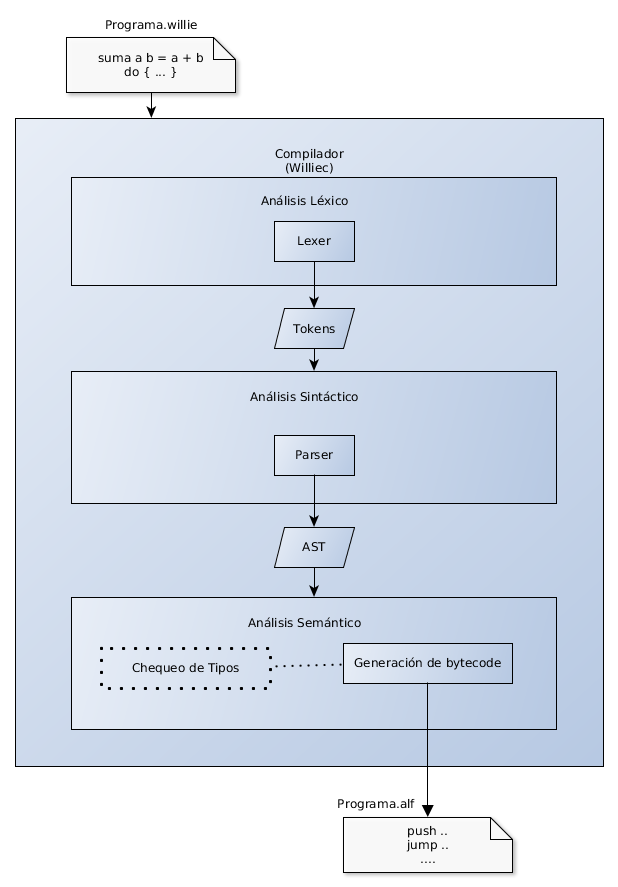
\includegraphics[width=0.9\textwidth]{graphs/compiler.png}
\label{fig:compiler}
\end{center}
\end{figure}


